
\documentclass[12pt,a4paper]{article}

% ------------------------------------------------------------
% Fonts & layout
% ------------------------------------------------------------
\usepackage[T1]{fontenc}
\usepackage[utf8]{inputenc}
\usepackage{lmodern}
\usepackage{microtype}
\usepackage{geometry}
\geometry{margin=1in}
\usepackage{array}
\usepackage{booktabs}

% ------------------------------------------------------------
% Math
% ------------------------------------------------------------
\usepackage{amsmath,amssymb,amsthm,mathtools}

% Standard operators
\DeclareMathOperator{\id}{id}
\DeclareMathOperator{\im}{im}
\DeclareMathOperator{\coker}{coker}
\DeclareMathOperator{\Hom}{Hom}

\DeclareMathOperator{\Spec}{Spec}
\DeclareMathOperator{\Proj}{Proj}

% Categories / notation
\newcommand{\Ab}{\mathbf{Ab}}
\newcommand{\PreSh}{\mathbf{PreSh}}
\newcommand{\Sh}{\mathbf{Sh}}

\newcommand{\F}{\mathcal F}


% basic number sets
\newcommand{\RR}{\mathbb{R}}

% sheaf letters

\newcommand{\G}{\mathcal G}

\newcommand{\GG}{\mathbb G}


\newcommand{\AffSch}{\mathbf{AffSch}}
\newcommand{\ZZ}{\mathbb Z}

\newcommand{\PP}{\mathbb P}

\usepackage{tikz}
\usetikzlibrary{decorations.pathreplacing}
\usetikzlibrary{positioning,arrows.meta}

% sheaf of continuous real-valued functions
\newcommand{\Czero}{\mathcal C^0}        % “C^0”
\newcommand{\CzeroX}{\mathcal C^0_X}     % sheaf on X (optional)

\newcommand{\Cinfty}{\mathcal C^\infty}
\newcommand{\CinftyM}{\mathcal C^\infty_M} % if you use C^\infty_M

% number sets / standard symbols
\newcommand{\CC}{\mathbb{C}}

% structure sheaf notation in complex geometry
\newcommand{\OO}{\mathcal{O}}
\newcommand{\OOX}{\mathcal{O}_X} % optional convenience



\newcommand{\Sch}{\mathrm{Sch}}
\newcommand{\Rings}{\mathrm{Rings}}

\newcommand{\kappares}{\kappa}
\newcommand{\GammaX}{\Gamma(X,\mathcal O_X)}

\newtheorem{theorem}{Theorem}[section]
\newtheorem{proposition}[theorem]{Proposition}
\newtheorem{lemma}[theorem]{Lemma}

\newcommand{\nilrad}{\sqrt{(0)}}

\newcommand{\Frac}{\operatorname{Frac}}
\newcommand{\codim}{\operatorname{codim}}
\newcommand{\trdeg}{\operatorname{trdeg}}

\newcommand{\height}{\operatorname{height}}

\newcommand{\Pic}{\operatorname{Pic}}
\newcommand{\divisor}{\operatorname{div}}

\newcommand{\Z}{\mathbb{Z}}
\newcommand{\Cl}{\operatorname{Cl}}

\providecommand{\Spec}{\operatorname{Spec}}
\providecommand{\A}{\mathbb A}
\providecommand{\Pj}{\mathbb P}
\providecommand{\G}{\mathbb G}

% ------------------------------------------------------------
% Links
% ------------------------------------------------------------
\usepackage{xcolor}
\usepackage{hyperref}
\usepackage{bookmark}
\hypersetup{
  colorlinks=true,
  linkcolor=blue!50!black,
  urlcolor=blue!50!black,
  citecolor=blue!50!black,
  pdftitle={Algebraic Geometry 15
  },
  pdfauthor={},
  pdfsubject={Lecture notes (reorganized)},
  pdfcreator={TeXStudio / LaTeX}
}

% ------------------------------------------------------------
% Diagrams
% ------------------------------------------------------------
\usepackage{tikz-cd}

% ------------------------------------------------------------
% Lists
% ------------------------------------------------------------
\usepackage{enumitem}
\setlist[itemize]{topsep=4pt,itemsep=2pt,parsep=0pt,partopsep=0pt}
\setlist[enumerate]{topsep=4pt,itemsep=2pt,parsep=0pt,partopsep=0pt}

% ------------------------------------------------------------
% Theorem environments
% ------------------------------------------------------------
\newtheoremstyle{notespace}{6pt}{6pt}{\normalfont}{}{\bfseries}{.}{0.5em}{}
\theoremstyle{notespace}
\newtheorem{definition}{Definition}[subsection]

\newtheorem{corollary}[definition]{Corollary}
\newtheorem{remark}[definition]{Remark}
\newtheorem{example}[definition]{Example}
\newtheorem{warning}[definition]{Warning}


\DeclareMathOperator{\Log}{Log}

\newcommand{\B}{\mathcal B}
\newcommand{\C}{\mathcal C}
\newcommand{\Ocal}{\mathcal O}
\newcommand{\I}{\mathcal I}


\newcommand{\Fp}{\mathcal F'}      % subsheaf
\newcommand{\Fpp}{\mathcal F''} 

\newcommand{\GammaU}[1]{\Gamma(U,#1)}

\DeclareMathOperator*{\colim}{colim}

% circle
\newcommand{\SSone}{S^1}


\usetikzlibrary{arrows.meta,positioning,calc,shapes.geometric,fit}

\usepackage{adjustbox}

% sheaves of continuous functions


% ------------------------------------------------------------
% Paragraph spacing
% ------------------------------------------------------------
\setlength{\parskip}{0.5em}
\setlength{\parindent}{0pt}

\setcounter{tocdepth}{2}
\setcounter{secnumdepth}{2}

% ------------------------------------------------------------
% Fancy headers
% ------------------------------------------------------------
\usepackage{fancyhdr}
\pagestyle{fancy}
\fancyhf{}
\lhead{Theory of Algebraic Geometry 15}
\rhead{\thepage}
\renewcommand{\headrulewidth}{0.4pt}
\setlength{\headheight}{14.5pt}




\begin{document}


\title{Algebraic Geometry 15\\
	\large Riemann surfaces}
\author{}
\date{}

	\maketitle
	

	\setcounter{section}{0}

\tableofcontents

	\clearpage
	
\section{Problem 6: The Riemann Surface of \texorpdfstring{$(z^4-1)^{1/4}$}{(z4-1)1/4}}

\subsection*{Problem statement}

Let
\[
\pi:R\to \mathbb C\setminus\{1,i,-1,-i\}
\]
be the Riemann surface associated to the complete analytic function
\[
(z^4-1)^{1/4}.
\]
Describe \(R\) explicitly by a gluing construction. Assuming the fact that
\(R\) may be compactified to a compact Riemann surface \(\overline R\) and
\(\pi\) extended to an analytic map
\[
\overline \pi:\overline R\to \mathbb C_\infty,
\]
find the genus of \(\overline R\).

\subsection*{Solution}

We study the multivalued function
\[
w=(z^4-1)^{1/4}.
\]
Equivalently, its compactified Riemann surface is the smooth projective model
of the affine curve
\[
w^4=z^4-1.
\]

The branch points in the finite \(z\)-plane are the roots of
\[
z^4-1=0,
\]
namely
\[
1,\quad i,\quad -1,\quad -i.
\]

Away from these four points, the equation
\[
w^4=z^4-1
\]
has four distinct values of \(w\). Therefore over
\[
\mathbb C\setminus\{1,i,-1,-i\}
\]
the surface is a four-sheeted covering.

Choose four copies
\[
S_0,S_1,S_2,S_3
\]
of the cut plane
\[
\mathbb C\setminus\Gamma,
\]
where \(\Gamma\) is a system of cuts joining the branch points. For example,
we may take cuts joining the points cyclically:
\[
1\longleftrightarrow i,\qquad
i\longleftrightarrow -1,\qquad
-1\longleftrightarrow -i,\qquad
-i\longleftrightarrow 1.
\]

On the \(k\)-th sheet we choose the branch
\[
w_k(z)=e^{2\pi i k/4}(z^4-1)^{1/4}
=i^k(z^4-1)^{1/4},
\qquad k=0,1,2,3.
\]

When one analytically continues once around any branch point, the value of
\((z^4-1)^{1/4}\) is multiplied by
\[
e^{2\pi i/4}=i.
\]
Thus the monodromy sends
\[
S_k\longmapsto S_{k+1},
\]
with indices taken modulo \(4\).

Hence the gluing rule is:

\[
\boxed{
	\text{the upper bank of each cut on }S_k
	\text{ is glued to the lower bank of the same cut on }S_{k+1}.
}
\]

Equivalently, the four sheets are glued cyclically:
\[
S_0\to S_1\to S_2\to S_3\to S_0.
\]

Near a branch point \(a\in\{1,i,-1,-i\}\), we have
\[
z^4-1=(z-a)u(z),
\]
where \(u(a)\neq 0\). Therefore locally
\[
w^4=(z-a)u(z).
\]
After absorbing the unit \(u(z)\), this has the local form
\[
z-a=t^4.
\]
So over each branch point there is one ramification point with ramification
index
\[
e=4.
\]

There are four such branch points. Therefore the total ramification
contribution is
\[
4(e-1)=4(4-1)=12.
\]

The map
\[
\overline\pi:\overline R\to\mathbb C_\infty
\]
has degree \(4\). By the Riemann--Hurwitz formula,
\[
2g(\overline R)-2
=
4(2g(\mathbb C_\infty)-2)
+
\sum_P(e_P-1).
\]
Since
\[
g(\mathbb C_\infty)=0,
\]
we get
\[
2g(\overline R)-2
=
4(-2)+12.
\]
Thus
\[
2g(\overline R)-2=4,
\]
so
\[
2g(\overline R)=6,
\]
and therefore
\[
\boxed{g(\overline R)=3.}
\]

Thus the compactified Riemann surface of
\[
(z^4-1)^{1/4}
\]
has genus \(3\).	
	
\section{Problem 7: Classification of Discrete Additive Subgroups of \texorpdfstring{$\mathbb C$}{C}}

\subsection*{Problem statement}

Suppose \(\Omega\subseteq\mathbb C\) is a discrete additive subgroup.
Here, discrete means that the subspace topology on \(\Omega\) is discrete.
Show that one of the following holds:

\[
\text{(i)}\quad \Omega=\{0\},
\]
or
\[
\text{(ii)}\quad \Omega=\mathbb Z\omega
\quad\text{for some }\omega\neq 0,
\]
or
\[
\text{(iii)}\quad
\Omega=\mathbb Z\omega_1+\mathbb Z\omega_2
\]
with
\[
\omega_1,\omega_2\neq 0
\]
and
\[
\omega_2/\omega_1\notin\mathbb R.
\]

\subsection*{Solution}

We identify
\[
\mathbb C\cong \mathbb R^2.
\]
Thus \(\Omega\) is a discrete additive subgroup of the real vector space
\(\mathbb R^2\).

If
\[
\Omega=\{0\},
\]
we are in case (i).

Assume now that
\[
\Omega\neq\{0\}.
\]
Since \(\Omega\) is discrete, there exists a nonzero element of minimal length.
Choose
\[
\omega_1\in\Omega,\qquad \omega_1\neq 0,
\]
such that
\[
|\omega_1|\leq |\omega|
\]
for every nonzero \(\omega\in\Omega\).

First suppose that every element of \(\Omega\) lies on the real line spanned
by \(\omega_1\). Then
\[
\Omega\subseteq \mathbb R\omega_1.
\]
We claim that
\[
\Omega=\mathbb Z\omega_1.
\]

Indeed, take any \(\omega\in\Omega\). Since \(\omega\in\mathbb R\omega_1\),
there exists \(t\in\mathbb R\) such that
\[
\omega=t\omega_1.
\]
Choose \(n\in\mathbb Z\) such that
\[
t-n\in\left[-\frac12,\frac12\right].
\]
Then
\[
\omega-n\omega_1=(t-n)\omega_1\in\Omega.
\]
But
\[
|\omega-n\omega_1|\leq \frac12|\omega_1|.
\]
By minimality of \(\omega_1\), this is possible only if
\[
\omega-n\omega_1=0.
\]
Therefore
\[
\omega=n\omega_1.
\]
Hence
\[
\Omega=\mathbb Z\omega_1,
\]
which is case (ii).

Now suppose that \(\Omega\) contains an element not lying on
\[
\mathbb R\omega_1.
\]
Then choose
\[
\omega_2\in\Omega\setminus\mathbb R\omega_1
\]
with minimal positive distance from the line \(\mathbb R\omega_1\).
This is possible because \(\Omega\) is discrete.

We claim that
\[
\Omega=\mathbb Z\omega_1+\mathbb Z\omega_2.
\]

Let \(\omega\in\Omega\). Since \(\omega_1,\omega_2\) are linearly independent
over \(\mathbb R\), there exist real numbers \(a,b\) such that
\[
\omega=a\omega_1+b\omega_2.
\]
Choose integers \(m,n\in\mathbb Z\) such that
\[
a-m\in\left[-\frac12,\frac12\right],
\qquad
b-n\in\left[-\frac12,\frac12\right].
\]
Then
\[
\eta=\omega-m\omega_1-n\omega_2\in\Omega.
\]
Moreover, \(\eta\) lies in a bounded fundamental parallelogram spanned by
\(\omega_1,\omega_2\).

If \(\eta\neq 0\), then by subtracting suitable integer multiples of
\(\omega_1\), one would obtain a nonzero element of \(\Omega\) either shorter
than \(\omega_1\) in the direction of \(\omega_1\), or with smaller positive
distance from the line \(\mathbb R\omega_1\) than \(\omega_2\). This contradicts
the choices of \(\omega_1\) and \(\omega_2\).

Hence
\[
\eta=0.
\]
Therefore
\[
\omega=m\omega_1+n\omega_2.
\]
So
\[
\Omega=\mathbb Z\omega_1+\mathbb Z\omega_2.
\]

Because \(\omega_2\notin\mathbb R\omega_1\), we have
\[
\omega_2/\omega_1\notin\mathbb R.
\]

Therefore \(\Omega\) is either trivial, cyclic, or a rank-two lattice:
\[
\boxed{
	\Omega=\{0\},
	\quad
	\Omega=\mathbb Z\omega,
	\quad\text{or}\quad
	\Omega=\mathbb Z\omega_1+\mathbb Z\omega_2
	\text{ with }\omega_2/\omega_1\notin\mathbb R.
}
\]
	
\section{Problem 8: Finite Fourier Expansion of a Simply Periodic Analytic Function}

\subsection*{Problem statement}

Let \(f\) be a simply periodic analytic function on \(\mathbb C\) with periods
\(\mathbb Z\). Suppose furthermore that
\[
f(x+iy)
\]
converges uniformly in \(x\) to possibly infinite limits as
\[
y\to\pm\infty.
\]
Show that
\[
f(z)=\sum_{k=-n}^{m} a_k e^{2\pi i kz},
\]
i.e. \(f(z)\) has a finite Fourier expansion.

\subsection*{Solution}

Since \(f\) has periods \(\mathbb Z\), we have
\[
f(z+1)=f(z).
\]
Therefore \(f\) descends to an analytic function on the punctured plane
\[
\mathbb C^*.
\]

Define
\[
q=e^{2\pi i z}.
\]
If
\[
z=x+iy,
\]
then
\[
|q|=|e^{2\pi i(x+iy)}|=e^{-2\pi y}.
\]
Hence
\[
y\to+\infty
\quad\Longleftrightarrow\quad
q\to 0,
\]
and
\[
y\to-\infty
\quad\Longleftrightarrow\quad
q\to\infty.
\]

Because \(f\) is \(1\)-periodic, there exists an analytic function
\[
F:\mathbb C^*\to\mathbb C
\]
such that
\[
f(z)=F(q)=F(e^{2\pi i z}).
\]

The assumption that \(f(x+iy)\) converges uniformly in \(x\) as
\(y\to+\infty\) says that \(F(q)\) has a limit as
\[
q\to 0.
\]
This limit is allowed to be infinite. Therefore \(q=0\) is either a removable
singularity or a pole of \(F\).

Similarly, the assumption that \(f(x+iy)\) converges uniformly in \(x\) as
\(y\to-\infty\) says that \(F(q)\) has a limit as
\[
q\to\infty.
\]
Thus \(q=\infty\) is either a removable singularity or a pole of \(F\).

Therefore \(F\) is meromorphic on the Riemann sphere
\[
\mathbb C_\infty
\]
with possible poles only at
\[
0
\quad\text{and}\quad
\infty.
\]

A meromorphic function on \(\mathbb C_\infty\) with poles only at \(0\) and
\(\infty\) is a Laurent polynomial. Hence there exist integers \(m,n\geq 0\)
and constants \(a_k\in\mathbb C\) such that
\[
F(q)=\sum_{k=-n}^{m}a_kq^k.
\]
Substituting
\[
q=e^{2\pi i z},
\]
we obtain
\[
f(z)
=
F(e^{2\pi i z})
=
\sum_{k=-n}^{m}a_k e^{2\pi i kz}.
\]

Thus \(f\) has a finite Fourier expansion:
\[
\boxed{
	f(z)=\sum_{k=-n}^{m}a_k e^{2\pi i kz}.
}
\]

\section{Problem 9: Zeros and Poles of an Elliptic Function}

\subsection*{Problem statement}

Let \(f\) be a non-constant elliptic function with respect to a lattice
\[
\Lambda\subset\mathbb C,
\]
and let \(P\subset\mathbb C\) be a fundamental parallelogram. Using the
argument principle and, if necessary, slightly perturbing \(P\), show that
the number of zeros of \(f\) in \(P\) is the same as the number of poles, both
counted with multiplicities.

This is also a consequence of the valency theorem, but the point of this
question is that this more direct argument via contour integration also works.

\subsection*{Solution}

Let
\[
\Lambda=\mathbb Z\omega_1+\mathbb Z\omega_2,
\]
where
\[
\omega_2/\omega_1\notin\mathbb R.
\]
A fundamental parallelogram is
\[
P=\{a+s\omega_1+t\omega_2:0\leq s,t\leq 1\}.
\]

Because \(f\) is elliptic with respect to \(\Lambda\), we have
\[
f(z+\omega)=f(z)
\]
for every
\[
\omega\in\Lambda.
\]
In particular,
\[
f(z+\omega_1)=f(z),
\qquad
f(z+\omega_2)=f(z).
\]

If necessary, slightly translate the parallelogram \(P\) so that no zero or
pole of \(f\) lies on its boundary. This is possible because zeros and poles
of a meromorphic function are isolated.

By the argument principle,
\[
N-P
=
\frac{1}{2\pi i}\int_{\partial P}\frac{f'(z)}{f(z)}\,dz,
\]
where \(N\) is the number of zeros of \(f\) inside \(P\), counted with
multiplicity, and \(P\) is the number of poles of \(f\) inside \(P\), counted
with multiplicity.

We now show that the boundary integral is zero.

The boundary of the parallelogram consists of four sides. Opposite sides are
translations of each other by periods. Since
\[
f(z+\omega_j)=f(z),
\]
we also have
\[
f'(z+\omega_j)=f'(z).
\]
Therefore
\[
\frac{f'(z+\omega_j)}{f(z+\omega_j)}
=
\frac{f'(z)}{f(z)}.
\]
Thus the logarithmic derivative
\[
\frac{f'}{f}
\]
is also elliptic with respect to the same lattice.

Now consider the two opposite sides parallel to \(\omega_1\). They are
translated versions of one another by \(\omega_2\), but they are traversed in
opposite directions in the boundary orientation. Since \(\frac{f'}{f}\) is
periodic, their integrals cancel.

Similarly, the two opposite sides parallel to \(\omega_2\) are translated
versions of one another by \(\omega_1\), again traversed in opposite
directions. Their integrals also cancel.

Therefore
\[
\int_{\partial P}\frac{f'(z)}{f(z)}\,dz=0.
\]

Hence the argument principle gives
\[
N-P=0.
\]
Therefore
\[
N=P.
\]

Thus the number of zeros of \(f\) in a fundamental parallelogram equals the
number of poles, counted with multiplicities:
\[
\boxed{
	\#\{\text{zeros of }f\text{ in }P\}
	=
	\#\{\text{poles of }f\text{ in }P\}.
}
\]
	
\section{Theory Behind Problems 6--9: Branched Coverings, Lattices, Fourier Expansions, and Elliptic Functions}

Problems 6--9 form a natural progression through several of the central ideas of complex analysis and Riemann surface theory:

\[
\text{Riemann Surfaces}
\longrightarrow
\text{Branched Coverings}
\longrightarrow
\text{Lattices}
\longrightarrow
\text{Complex Tori}
\longrightarrow
\text{Periodic Functions}
\longrightarrow
\text{Elliptic Functions}.
\]

These concepts eventually lead to elliptic curves, algebraic geometry, modular forms, and number theory.

\subsection{Branched Coverings and Multivalued Functions}

Many complex functions are naturally multivalued. Examples include

\[
\sqrt{z},
\qquad
\log z,
\qquad
(z^4-1)^{1/4}.
\]

For instance,

\[
w=(z^4-1)^{1/4}
\]

satisfies

\[
w^4=z^4-1.
\]

At a generic point \(z\), there are four possible values of \(w\):

\[
w,\quad iw,\quad -w,\quad -iw.
\]

To make the function single-valued we construct a Riemann surface consisting of four sheets glued together appropriately.

\subsection{Branch Points}

A branch point occurs where several sheets meet.

For

\[
w^4=z^4-1,
\]

branching occurs where

\[
z^4-1=0.
\]

Thus the branch points are

\[
1,\qquad i,\qquad -1,\qquad -i.
\]

Near such a point \(a\),

\[
w^4=z-a.
\]

Equivalently,

\[
z=a+w^4.
\]

The local model is therefore

\[
w\longmapsto w^4.
\]

Four sheets merge together at each branch point.

\subsection{Monodromy}

Monodromy describes what happens when one analytically continues a branch around a loop.

If we travel once around a branch point of

\[
(z^4-1)^{1/4},
\]

the value changes by

\[
w\mapsto iw.
\]

A second turn gives

\[
w\mapsto -w,
\]

a third turn gives

\[
w\mapsto -iw,
\]

and a fourth turn returns to the original branch.

Thus the monodromy permutation is

\[
(1\,2\,3\,4).
\]

Monodromy records how the sheets of a covering are glued together.

\subsection{Ramification}

The ramification index measures how many sheets come together.

If locally

\[
z=t^e,
\]

then the ramification index is \(e\).

Examples:

\[
z=t^2
\qquad\Rightarrow\qquad e=2,
\]

\[
z=t^3
\qquad\Rightarrow\qquad e=3,
\]

\[
z=t^4
\qquad\Rightarrow\qquad e=4.
\]

For Problem 6 each branch point has

\[
e=4.
\]

\subsection{The Riemann--Hurwitz Formula}

The genus of a branched covering is determined by the Riemann--Hurwitz formula:

\[
2g(X)-2
=
d\bigl(2g(Y)-2\bigr)
+
\sum_{P}(e_P-1),
\]

where

\begin{itemize}
	\item \(d\) is the degree of the covering,
	\item \(g(X)\) is the genus upstairs,
	\item \(g(Y)\) is the genus downstairs,
	\item \(e_P\) is the ramification index.
\end{itemize}

This formula shows precisely how branching creates additional handles on a surface.

For Problem 6:

\[
d=4,
\qquad
g(\mathbb P^1)=0,
\qquad
\sum(e_P-1)=4(4-1)=12.
\]

Hence

\[
2g-2=4(-2)+12=4,
\]

which gives

\[
g=3.
\]

Thus the compactified surface has genus three.

\subsection{Discrete Additive Subgroups of \(\mathbb C\)}

Problem 7 classifies discrete additive subgroups of \(\mathbb C\).

A subgroup

\[
\Omega\subseteq\mathbb C
\]

is discrete if every point is isolated.

The classification theorem states:

\[
\Omega=\{0\},
\]

or

\[
\Omega=\mathbb Z\omega,
\]

or

\[
\Omega=\mathbb Z\omega_1+\mathbb Z\omega_2,
\qquad
\omega_2/\omega_1\notin\mathbb R.
\]

No other possibilities exist.

Since

\[
\mathbb C\cong\mathbb R^2,
\]

the maximum rank of a discrete subgroup is \(2\).

\subsection{Lattices}

A lattice is a rank-two discrete subgroup

\[
\Lambda
=
\mathbb Z\omega_1
+
\mathbb Z\omega_2,
\]

where

\[
\omega_2/\omega_1\notin\mathbb R.
\]

Geometrically, lattice points form a repeating grid in the complex plane.

Examples:

\[
\Lambda=\mathbb Z+i\mathbb Z,
\]

(square lattice),

and

\[
\Lambda
=
\mathbb Z
+
e^{i\pi/3}\mathbb Z,
\]

(hexagonal lattice).

\subsection{Fundamental Parallelogram}

The fundamental parallelogram of a lattice is

\[
P=
\{
s\omega_1+t\omega_2:
0\le s,t\le1
\}.
\]

Every point of \(\mathbb C\) is congruent modulo \(\Lambda\) to exactly one point of \(P\).

The complex plane is tiled by translated copies of \(P\).

\begin{center}
	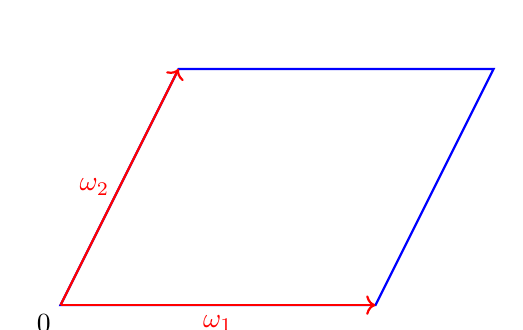
\begin{tikzpicture}[scale=1]
		
		\coordinate (A) at (0,0);
		\coordinate (B) at (4,0);
		\coordinate (D) at (1.5,3);
		\coordinate (C) at (5.5,3);
		
		\draw[thick,blue] (A)--(B)--(C)--(D)--cycle;
		
		\draw[->,red,thick] (A)--(B)
		node[midway,below] {$\omega_1$};
		
		\draw[->,red,thick] (A)--(D)
		node[midway,left] {$\omega_2$};
		
		\node[below left] at (A) {$0$};
		
	\end{tikzpicture}
\end{center}

\subsection{Complex Tori}

By identifying opposite sides of a fundamental parallelogram,

\[
\mathbb C/\Lambda,
\]

we obtain a compact Riemann surface.

First glue left and right edges to form a cylinder.

Then glue top and bottom edges.

The result is a torus.

\[
\boxed{
	\mathbb C/\Lambda
	\cong
	\text{torus}.
}
\]

This torus has genus

\[
g=1.
\]

\subsection{Periodic Functions}

A function is periodic if

\[
f(z+\omega)=f(z).
\]

If only one period exists, for example

\[
f(z+1)=f(z),
\]

the function is called simply periodic.

If two independent periods exist,

\[
f(z+\omega_1)=f(z),
\qquad
f(z+\omega_2)=f(z),
\]

the function is doubly periodic.

\subsection{Fourier Expansions}

For a \(1\)-periodic analytic function,

\[
f(z+1)=f(z),
\]

we introduce

\[
q=e^{2\pi iz}.
\]

Then

\[
z\sim z+1
\]

corresponds to the same value of \(q\).

Every periodic analytic function has a Fourier expansion

\[
f(z)
=
\sum_{k=-\infty}^{\infty}
a_k e^{2\pi ikz}.
\]

Equivalently,

\[
f(z)
=
\sum_{k=-\infty}^{\infty}
a_k q^k.
\]

\subsection{Finite Fourier Expansions}

Problem 8 assumes controlled behaviour as

\[
y\to\pm\infty.
\]

Since

\[
q=e^{2\pi iz},
\]

we have

\[
y\to+\infty
\Longleftrightarrow
q\to0,
\]

and

\[
y\to-\infty
\Longleftrightarrow
q\to\infty.
\]

The assumptions imply that \(q=0\) and \(q=\infty\) are at worst poles.

Hence only finitely many positive and negative powers occur.

Therefore

\[
f(z)
=
\sum_{k=-n}^{m}
a_k e^{2\pi ikz}.
\]

Thus \(f\) is represented by a finite Laurent polynomial in \(q\).

\subsection{Elliptic Functions}

An elliptic function is a meromorphic function satisfying

\[
f(z+\omega_1)=f(z),
\qquad
f(z+\omega_2)=f(z),
\]

for a lattice

\[
\Lambda
=
\mathbb Z\omega_1
+
\mathbb Z\omega_2.
\]

Hence elliptic functions are precisely meromorphic functions on

\[
\mathbb C/\Lambda.
\]

Since

\[
\mathbb C/\Lambda
\]

is a torus, we obtain:

\[
\boxed{
	\text{Elliptic functions}
	=
	\text{meromorphic functions on a torus}.
}
\]

This is one of the most important ideas in complex analysis.

\subsection{The Argument Principle}

If \(f\) is meromorphic inside a contour \(\gamma\), then

\[
\frac{1}{2\pi i}
\int_{\gamma}
\frac{f'(z)}{f(z)}
\,dz
=
N-P,
\]

where

\begin{itemize}
	\item \(N\) is the number of zeros,
	\item \(P\) is the number of poles,
\end{itemize}

counted with multiplicities.

The logarithmic derivative

\[
\frac{f'}{f}
\]

records the net number of zeros minus poles.

\subsection{Zeros and Poles of Elliptic Functions}

Let \(P\) be a fundamental parallelogram.

Because

\[
f(z+\omega_j)=f(z),
\]

the logarithmic derivative is also periodic:

\[
\frac{f'(z+\omega_j)}
{f(z+\omega_j)}
=
\frac{f'(z)}
{f(z)}.
\]

Opposite sides of \(P\) contribute equal integrals with opposite orientations.

Therefore

\[
\int_{\partial P}
\frac{f'}{f}\,dz
=
0.
\]

Applying the argument principle gives

\[
N-P=0.
\]

Hence

\[
\boxed{
	N=P.
}
\]

An elliptic function has exactly as many zeros as poles in a fundamental parallelogram, counted with multiplicities.

\subsection{The Valency Theorem}

A stronger result states

\[
\sum_{a\in P}
\operatorname{ord}_a(f)
=
0.
\]

Positive orders correspond to zeros.

Negative orders correspond to poles.

Thus the total multiplicity of zeros equals the total multiplicity of poles.

Problem 9 is essentially a direct proof of this theorem using contour integration.

\subsection{Conceptual Summary}

\[
\text{Branch Points}
\longrightarrow
\text{Ramification}
\longrightarrow
\text{Riemann Surfaces}
\longrightarrow
\text{Riemann--Hurwitz}
\]

\[
\text{Discrete Subgroups}
\longrightarrow
\text{Lattices}
\longrightarrow
\text{Fundamental Parallelograms}
\longrightarrow
\text{Complex Tori}
\]

\[
\text{Periodic Functions}
\longrightarrow
\text{Fourier Series}
\longrightarrow
\text{Elliptic Functions}
\]

\[
\text{Elliptic Functions}
\longrightarrow
\text{Argument Principle}
\longrightarrow
\text{Valency Theorem}
\longrightarrow
\text{Elliptic Curves}.
\]

These ideas form one of the principal bridges between complex analysis, topology, Riemann surfaces, and modern algebraic geometry.	

\section{Introduction to Modular Forms}

The theory of modular forms is one of the deepest continuations of the theory of lattices, complex tori, and elliptic functions.

The chain of ideas is

\[
\text{Lattices}
\longrightarrow
\text{Complex Tori}
\longrightarrow
\text{Elliptic Functions}
\longrightarrow
\text{Modular Forms}
\longrightarrow
\text{Number Theory}.
\]

Historically, modular forms arose from the study of elliptic integrals and elliptic functions, but today they play central roles in algebraic geometry, arithmetic geometry, representation theory, and mathematical physics.

\subsection{The Upper Half-Plane}

The fundamental object is the upper half-plane

\[
\mathbb H
=
\{\tau\in\mathbb C:\operatorname{Im}(\tau)>0\}.
\]

Every lattice

\[
\Lambda
=
\mathbb Z\omega_1+\mathbb Z\omega_2
\]

may be rescaled so that

\[
\omega_1=1,
\qquad
\omega_2=\tau,
\]

with

\[
\tau\in\mathbb H.
\]

Thus every lattice can be written in the form

\[
\Lambda_\tau
=
\mathbb Z+\tau\mathbb Z.
\]

Consequently, points of \(\mathbb H\) parameterize complex tori

\[
\mathbb C/\Lambda_\tau.
\]

\subsection{Equivalent Lattices}

Different values of \(\tau\) may determine isomorphic tori.

For example,

\[
\Lambda_\tau
=
\mathbb Z+\tau\mathbb Z
\]

and

\[
\Lambda_{\tau+1}
=
\mathbb Z+(\tau+1)\mathbb Z
\]

define the same lattice.

Likewise,

\[
\Lambda_\tau
\quad\text{and}\quad
\Lambda_{-1/\tau}
\]

define equivalent complex tori.

These transformations generate the modular group

\[
SL_2(\mathbb Z)
=
\left\{
\begin{pmatrix}
	a&b\\
	c&d
\end{pmatrix}
:
a,b,c,d\in\mathbb Z,
\ ad-bc=1
\right\}.
\]

Its action on \(\mathbb H\) is

\[
\tau
\mapsto
\frac{a\tau+b}{c\tau+d}.
\]

\subsection{The Modular Group}

The modular group acts by biholomorphic transformations of the upper half-plane.

The two fundamental generators are

\[
T(\tau)=\tau+1,
\]

and

\[
S(\tau)=-\frac1\tau.
\]

Every element of \(SL_2(\mathbb Z)\) can be obtained from repeated compositions of \(S\) and \(T\).

The quotient space

\[
SL_2(\mathbb Z)\backslash\mathbb H
\]

classifies complex tori up to conformal equivalence.

Thus the moduli space of elliptic curves is essentially

\[
SL_2(\mathbb Z)\backslash\mathbb H.
\]

\subsection{Definition of a Modular Form}

A modular form of weight \(k\) is a holomorphic function

\[
f:\mathbb H\to\mathbb C
\]

satisfying

\[
f\!\left(
\frac{a\tau+b}{c\tau+d}
\right)
=
(c\tau+d)^k f(\tau)
\]

for every

\[
\begin{pmatrix}
	a&b\\
	c&d
\end{pmatrix}
\in SL_2(\mathbb Z),
\]

and satisfying an additional regularity condition at infinity.

The factor

\[
(c\tau+d)^k
\]

is called the automorphy factor.

\subsection{The Cusp at Infinity}

The point

\[
\tau=i\infty
\]

is called the cusp at infinity.

Because modular forms satisfy

\[
f(\tau+1)=f(\tau),
\]

they are periodic.

We therefore introduce

\[
q=e^{2\pi i\tau}.
\]

This converts periodicity into ordinary power series.

A modular form has a Fourier expansion

\[
f(\tau)
=
\sum_{n=0}^{\infty}
a_n q^n.
\]

This is called the \(q\)-expansion.

The coefficients \(a_n\) often contain deep arithmetic information.

\subsection{Cusp Forms}

If

\[
a_0=0,
\]

then \(f\) is called a cusp form.

Equivalently,

\[
f(i\infty)=0.
\]

Cusp forms vanish at the cusp and form one of the most important spaces in number theory.

\subsection{Eisenstein Series}

The simplest modular forms are Eisenstein series.

For even integers \(k\ge 4\),

\[
G_k(\tau)
=
\sum_{(m,n)\neq(0,0)}
\frac1{(m+n\tau)^k}.
\]

These series converge absolutely and define modular forms of weight \(k\).

Examples:

\[
G_4(\tau),
\qquad
G_6(\tau).
\]

Every classical modular form can ultimately be built from these.

\subsection{The Modular Discriminant}

One of the most important cusp forms is

\[
\Delta(\tau)
=
q
\prod_{n=1}^{\infty}
(1-q^n)^{24}.
\]

Its Fourier expansion begins

\[
\Delta(\tau)
=
q
-
24q^2
+
252q^3
-
1472q^4
+\cdots.
\]

This is a cusp form of weight \(12\).

The coefficients of \(\Delta\) contain profound arithmetic information.

\subsection{The Modular \(j\)-Invariant}

A central object is the modular invariant

\[
j(\tau).
\]

It is constructed from Eisenstein series and the discriminant:

\[
j(\tau)
=
1728
\frac{G_4(\tau)^3}
{G_4(\tau)^3-27G_6(\tau)^2}.
\]

The remarkable theorem is:

\[
j(\tau_1)=j(\tau_2)
\]

if and only if

\[
\Lambda_{\tau_1}
\]

and

\[
\Lambda_{\tau_2}
\]

define isomorphic complex tori.

Thus \(j\) completely classifies elliptic curves over \(\mathbb C\).

\subsection{Connection with Elliptic Curves}

Every lattice

\[
\Lambda
\]

determines an elliptic curve

\[
E_\Lambda
=
\mathbb C/\Lambda.
\]

Using the Weierstrass \(\wp\)-function,

\[
\wp(z),
\]

one obtains an algebraic equation

\[
y^2
=
4x^3
-
g_2x
-
g_3.
\]

The coefficients

\[
g_2,
\qquad
g_3
\]

are modular forms.

Thus modular forms naturally describe families of elliptic curves.

\subsection{Modular Forms and Number Theory}

One reason modular forms are so important is that their Fourier coefficients encode arithmetic information.

Examples include:

\begin{itemize}
	\item partitions,
	\item divisor sums,
	\item representations by quadratic forms,
	\item class numbers,
	\item values of \(L\)-functions,
	\item arithmetic of elliptic curves.
\end{itemize}

Many famous number-theoretic identities arise from modular forms.

\subsection{The Modularity Theorem}

A milestone of modern mathematics is the Modularity Theorem.

It states that every elliptic curve over \(\mathbb Q\) is associated with a modular form.

Symbolically,

\[
\text{Elliptic Curve}
\longleftrightarrow
\text{Modular Form}.
\]

This theorem was the key ingredient in the proof of Fermat's Last Theorem.

\subsection{Geometric Picture}

The progression of ideas can be visualized as

\[
\tau\in\mathbb H
\]

\[
\Downarrow
\]

\[
\Lambda_\tau
=
\mathbb Z+\tau\mathbb Z
\]

\[
\Downarrow
\]

\[
\mathbb C/\Lambda_\tau
\]

\[
\Downarrow
\]

\[
\text{Complex Torus}
\]

\[
\Downarrow
\]

\[
\text{Elliptic Curve}
\]

\[
\Downarrow
\]

\[
\text{Modular Forms}
\]

\[
\Downarrow
\]

\[
\text{Arithmetic Information}.
\]

\subsection{Conceptual Summary}

\[
\text{Discrete Subgroups}
\longrightarrow
\text{Lattices}
\]

\[
\text{Lattices}
\longrightarrow
\text{Complex Tori}
\]

\[
\text{Complex Tori}
\longrightarrow
\text{Elliptic Functions}
\]

\[
\text{Elliptic Functions}
\longrightarrow
\text{Elliptic Curves}
\]

\[
\text{Elliptic Curves}
\longrightarrow
\text{Modular Forms}
\]

\[
\text{Modular Forms}
\longrightarrow
\text{Number Theory}.
\]

Modular forms may be viewed as functions on the space of all complex tori. They encode how elliptic curves vary, and their Fourier coefficients reveal some of the deepest arithmetic structures known in mathematics.


\section{Visual Diagrams, Tables, and Concept Maps for Problems 6--9}

\subsection{Roadmap of the Theory}

\begin{center}
	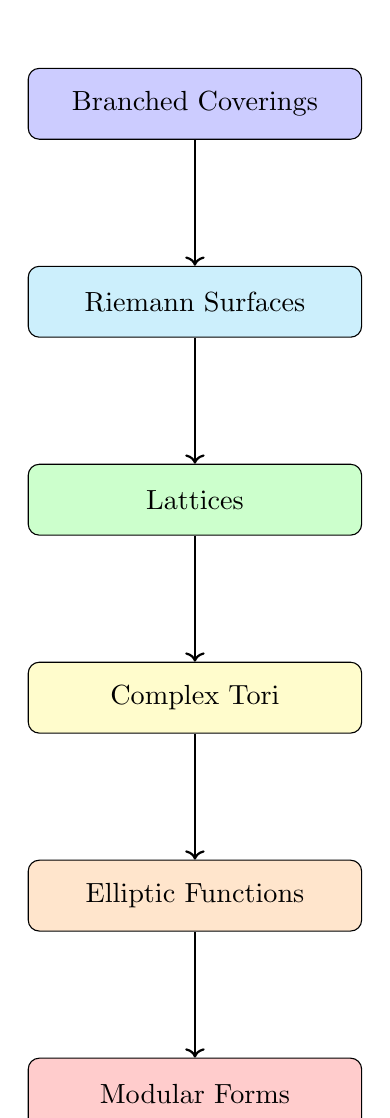
\begin{tikzpicture}[
		node distance=1.6cm,
		every node/.style={
			draw,
			rounded corners,
			align=center,
			text width=4cm,
			minimum height=0.9cm
		}
		]
		
		\node[fill=blue!20] (b)
		{Branched Coverings};
		
		\node[fill=cyan!20,below=of b] (r)
		{Riemann Surfaces};
		
		\node[fill=green!20,below=of r] (l)
		{Lattices};
		
		\node[fill=yellow!20,below=of l] (t)
		{Complex Tori};
		
		\node[fill=orange!20,below=of t] (e)
		{Elliptic Functions};
		
		\node[fill=red!20,below=of e] (m)
		{Modular Forms};
		
		\draw[->,thick] (b)--(r);
		\draw[->,thick] (r)--(l);
		\draw[->,thick] (l)--(t);
		\draw[->,thick] (t)--(e);
		\draw[->,thick] (e)--(m);
		
	\end{tikzpicture}
\end{center}


\subsection{Classification of Discrete Subgroups}

\begin{center}
	\renewcommand{\arraystretch}{1.4}
	\begin{tabular}{|c|c|c|c|}
		\hline
		Rank & Form & Geometry & Example\\
		\hline
		0 &
		\(\{0\}\) &
		Point &
		\(\{0\}\)
		\\
		\hline
		1 &
		\(\mathbb Z\omega\) &
		Line of points &
		\(\mathbb Z\)
		\\
		\hline
		2 &
		\(\mathbb Z\omega_1+\mathbb Z\omega_2\) &
		Lattice &
		\(\mathbb Z+i\mathbb Z\)
		\\
		\hline
	\end{tabular}
\end{center}


\subsection{Rank 1 Versus Rank 2}

\begin{center}
	
	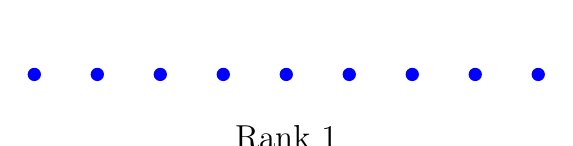
\begin{tikzpicture}[scale=0.8]
		
		\foreach \x in {-4,...,4}
		{
			\fill[blue] (\x,0) circle (3pt);
		}
		
		\node at (0,-1)
		{\large Rank 1};
		
	\end{tikzpicture}
	
	\vspace{1cm}
	
	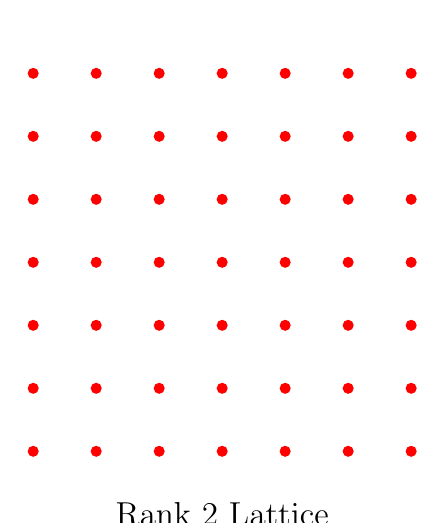
\begin{tikzpicture}[scale=0.8]
		
		\foreach \x in {-3,...,3}
		{
			\foreach \y in {-3,...,3}
			{
				\fill[red] (\x,\y) circle (2.5pt);
			}
		}
		
		\node at (0,-4)
		{\large Rank 2 Lattice};
		
	\end{tikzpicture}
	
\end{center}


\subsection{Fundamental Parallelogram}

\begin{center}
	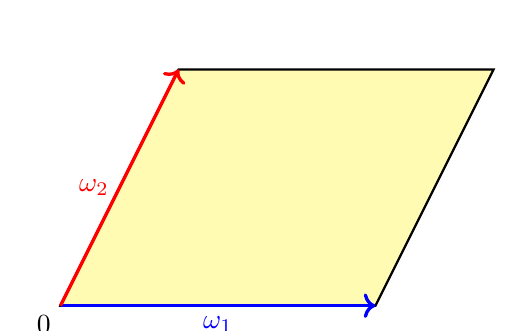
\begin{tikzpicture}[scale=1]
		
		\coordinate (A) at (0,0);
		\coordinate (B) at (4,0);
		\coordinate (D) at (1.5,3);
		\coordinate (C) at (5.5,3);
		
		\fill[yellow!30] (A)--(B)--(C)--(D)--cycle;
		
		\draw[thick] (A)--(B)--(C)--(D)--cycle;
		
		\draw[->,very thick,blue]
		(A)--(B)
		node[midway,below]
		{\(\omega_1\)};
		
		\draw[->,very thick,red]
		(A)--(D)
		node[midway,left]
		{\(\omega_2\)};
		
		\node[below left] at (A)
		{\(0\)};
		
	\end{tikzpicture}
\end{center}

The shaded region is one copy of the torus before edge identifications.


\subsection{From Parallelogram to Torus}

\begin{center}
	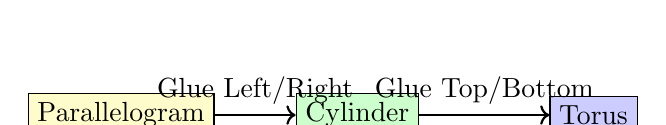
\begin{tikzpicture}[node distance=3cm]
		
		\node[draw,fill=yellow!20] (P)
		{Parallelogram};
		
		\node[draw,fill=green!20,right of=P]
		(C)
		{Cylinder};
		
		\node[draw,fill=blue!20,right of=C]
		(T)
		{Torus};
		
		\draw[->,thick]
		(P)--node[above]
		{Glue Left/Right}
		(C);
		
		\draw[->,thick]
		(C)--node[above]
		{Glue Top/Bottom}
		(T);
		
	\end{tikzpicture}
\end{center}



\subsection{Branching in Problem 6}

Branch points:

\[
1,\quad i,\quad -1,\quad -i.
\]

\begin{center}
	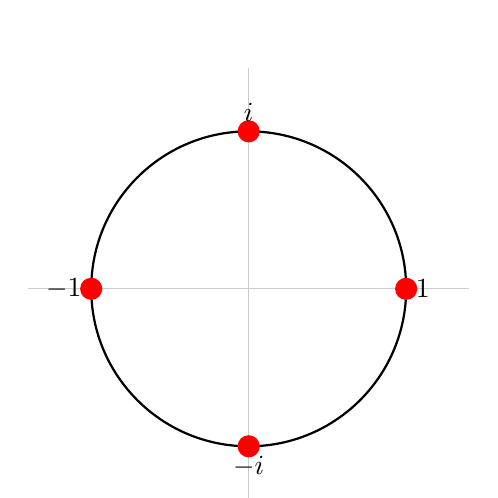
\begin{tikzpicture}[scale=2]
		
		\draw[gray!40] (-1.4,0)--(1.4,0);
		\draw[gray!40] (0,-1.4)--(0,1.4);
		
		\draw[thick] (0,0) circle (1);
		
		\fill[red] (1,0) circle (2pt);
		\fill[red] (-1,0) circle (2pt);
		\fill[red] (0,1) circle (2pt);
		\fill[red] (0,-1) circle (2pt);
		
		\node[right] at (1,0) {\(1\)};
		\node[left] at (-1,0) {\(-1\)};
		\node[above] at (0,1) {\(i\)};
		\node[below] at (0,-1) {\(-i\)};
		
	\end{tikzpicture}
\end{center}

Each red point is a branch point where four sheets meet.



\subsection{Monodromy of Problem 6}

\[
w=(z^4-1)^{1/4}
\]

A loop around any branch point produces

\[
w
\rightarrow
iw
\rightarrow
-w
\rightarrow
-iw
\rightarrow
w.
\]

\begin{center}
	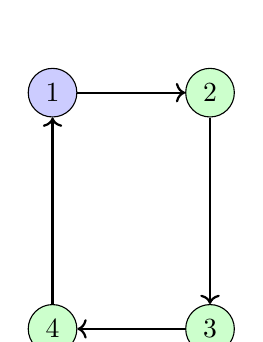
\begin{tikzpicture}[scale=1]
		
		\node[draw,circle,fill=blue!20] (1) at (0,1.5) {1};
		
		\node[draw,circle,fill=green!20] (2) at (2,1.5) {2};
		
		\node[draw,circle,fill=green!20] (3) at (2,-1.5) {3};
		
		\node[draw,circle,fill=green!20] (4) at (0,-1.5) {4};
		
		\draw[->,thick] (1)--(2);
		\draw[->,thick] (2)--(3);
		\draw[->,thick] (3)--(4);
		\draw[->,thick] (4)--(1);
		
	\end{tikzpicture}
\end{center}

Monodromy permutation:

\[
(1\,2\,3\,4).
\]



\subsection{Genus Comparison}

\begin{center}
	\renewcommand{\arraystretch}{1.4}
	\begin{tabular}{|c|c|c|}
		\hline
		Surface &
		Genus &
		Shape
		\\
		\hline
		Sphere &
		0 &
		No holes
		\\
		\hline
		Torus &
		1 &
		One hole
		\\
		\hline
		Double Torus &
		2 &
		Two holes
		\\
		\hline
		Problem 6 Surface &
		3 &
		Three holes
		\\
		\hline
	\end{tabular}
\end{center}



\subsection{Periodic and Elliptic Functions}

\begin{center}
	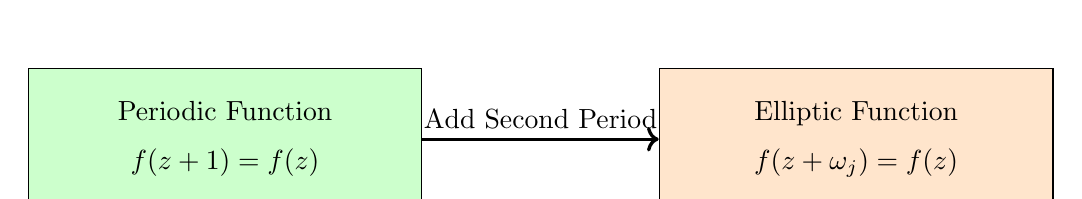
\begin{tikzpicture}
		
		\node[
		draw,
		fill=green!20,
		align=center,
		minimum width=5cm,
		minimum height=1.8cm
		] (P)
		{Periodic Function\\[2mm]
			\(f(z+1)=f(z)\)};
		
		\node[
		draw,
		fill=orange!20,
		align=center,
		minimum width=5cm,
		minimum height=1.8cm,
		right=3cm of P
		] (E)
		{Elliptic Function\\[2mm]
			\(f(z+\omega_j)=f(z)\)};
		
		\draw[->,very thick]
		(P) -- node[above]{Add Second Period} (E);
		
	\end{tikzpicture}
\end{center}



\subsection{Fourier Expansion}

For a periodic function:

\[
f(z)
=
\sum_{n=-\infty}^{\infty}
a_n e^{2\pi inz}.
\]

Problem 8 shows:

\[
f(z)
=
\sum_{n=-N}^{M}
a_n e^{2\pi inz}.
\]

only finitely many terms survive.

\begin{center}
	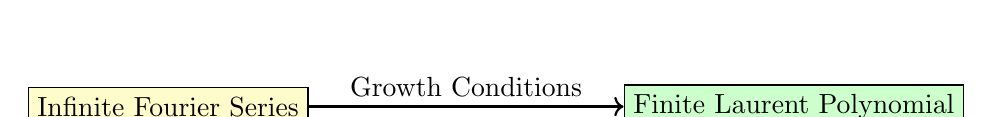
\begin{tikzpicture}
		
		\node[draw,fill=yellow!20]
		(A)
		{Infinite Fourier Series};
		
		\node[draw,fill=green!20,right=4cm of A]
		(B)
		{Finite Laurent Polynomial};
		
		\draw[->,thick]
		(A)--node[above]
		{Growth Conditions}
		(B);
		
	\end{tikzpicture}
\end{center}



\subsection{Zeros and Poles in a Fundamental Parallelogram}

Problem 9 proves

\[
N=P.
\]

\begin{center}
	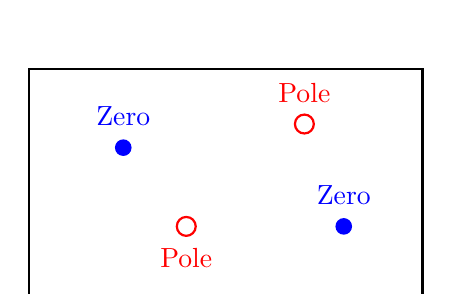
\begin{tikzpicture}[scale=1]
		
		\draw[thick]
		(0,0)
		rectangle
		(5,3);
		
		\fill[blue]
		(1.2,2)
		circle(3pt);
		
		\fill[blue]
		(4,1)
		circle(3pt);
		
		\draw[red,thick]
		(2,1)
		circle(0.12);
		
		\draw[red,thick]
		(3.5,2.3)
		circle(0.12);
		
		\node[blue] at (1.2,2.4)
		{Zero};
		
		\node[blue] at (4,1.4)
		{Zero};
		
		\node[red] at (2,0.6)
		{Pole};
		
		\node[red] at (3.5,2.7)
		{Pole};
		
	\end{tikzpicture}
\end{center}

The total multiplicity of zeros equals the total multiplicity of poles.



\subsection{Complete Concept Map}

\begin{center}
	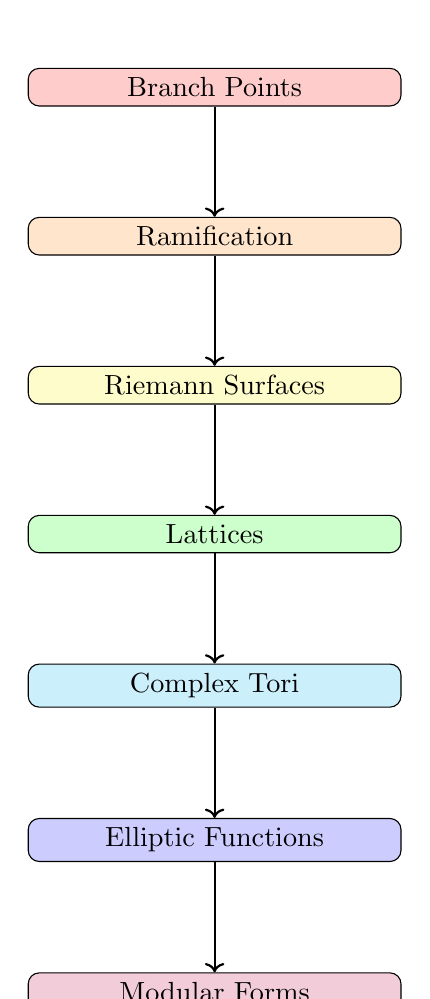
\begin{tikzpicture}[
		node distance=1.4cm,
		every node/.style={
			draw,
			rounded corners,
			align=center,
			text width=4.5cm
		}
		]
		
		\node[fill=red!20]
		(a)
		{Branch Points};
		
		\node[fill=orange!20,below=of a]
		(b)
		{Ramification};
		
		\node[fill=yellow!20,below=of b]
		(c)
		{Riemann Surfaces};
		
		\node[fill=green!20,below=of c]
		(d)
		{Lattices};
		
		\node[fill=cyan!20,below=of d]
		(e)
		{Complex Tori};
		
		\node[fill=blue!20,below=of e]
		(f)
		{Elliptic Functions};
		
		\node[fill=purple!20,below=of f]
		(g)
		{Modular Forms};
		
		\draw[->,thick] (a)--(b);
		\draw[->,thick] (b)--(c);
		\draw[->,thick] (c)--(d);
		\draw[->,thick] (d)--(e);
		\draw[->,thick] (e)--(f);
		\draw[->,thick] (f)--(g);
		
	\end{tikzpicture}
\end{center}

This diagram summarizes the entire mathematical journey from Problem 6 through Problem 9 and onward to modular forms.

	
\section{Sheaves, Presheaves, Sheafification, and Stalks}

\subsection{Motivation}

Many geometric and analytic objects are naturally defined only on open subsets of a space:

\begin{itemize}
	\item continuous functions,
	\item differentiable functions,
	\item holomorphic functions,
	\item vector fields,
	\item differential forms,
	\item solutions of differential equations.
\end{itemize}

A sheaf formalizes the principle that global information can be reconstructed from compatible local information.

\bigskip

\begin{center}
	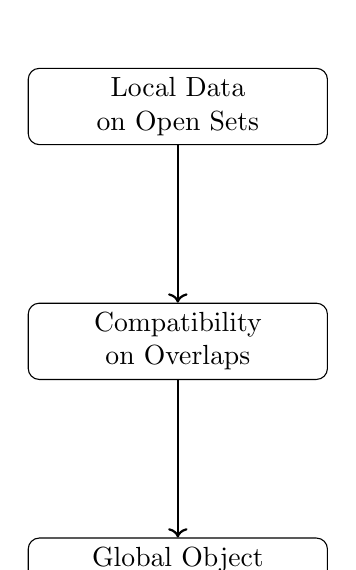
\begin{tikzpicture}[
		node distance=2cm,
		every node/.style={
			draw,
			rounded corners,
			align=center,
			minimum width=3.8cm
		}
		]
		
		\node (local) {Local Data\\on Open Sets};
		
		\node (compatible) [below=of local]
		{Compatibility\\on Overlaps};
		
		\node (global) [below=of compatible]
		{Global Object};
		
		\draw[->,thick] (local)--(compatible);
		\draw[->,thick] (compatible)--(global);
		
	\end{tikzpicture}
\end{center}

\subsection{Presheaves}

Let \(X\) be a topological space.

\begin{definition}[Presheaf]
	A \emph{presheaf} \(\mathcal F\) on \(X\) consists of
	
	\begin{enumerate}
		\item a set (or group, ring, module)
		\[
		\mathcal F(U)
		\]
		for every open subset \(U\subseteq X\),
		
		\item restriction maps
		\[
		\rho_{UV}:\mathcal F(U)\to\mathcal F(V)
		\]
		for every inclusion \(V\subseteq U\).
	\end{enumerate}
	
	These satisfy:
	
	\begin{enumerate}
		\item Identity:
		\[
		\rho_{UU}=id.
		\]
		
		\item Composition:
		if
		\[
		W\subseteq V\subseteq U,
		\]
		then
		\[
		\rho_{UW}
		=
		\rho_{VW}\circ \rho_{UV}.
		\]
	\end{enumerate}
\end{definition}

Usually we write

\[
s|_V
\]

instead of

\[
\rho_{UV}(s).
\]

\subsection{Restriction Diagram}

\begin{center}
	\begin{tikzpicture}[
		node distance=2.3cm,
		every node/.style={
			draw,
			rounded corners,
			minimum width=2cm
		}
		]
		
		\node (U) {\(U\)};
		\node (V) [below left=of U] {\(V\)};
		\node (W) [below right=of V] {\(W\)};
		
		\draw[->] (U)--(V);
		\draw[->] (V)--(W);
		\draw[->,bend left=25] (U)--(W);
		
	\end{tikzpicture}
\end{center}

The direct restriction

\[
U\to W
\]

equals the composition

\[
U\to V\to W.
\]

\subsection{Examples of Presheaves}

\subsubsection*{Continuous Functions}

\[
\mathcal C(U)
=
\{f:U\to\mathbb R \mid f \text{ continuous}\}.
\]

Restrictions are ordinary restrictions of functions.

\bigskip

\subsubsection*{Holomorphic Functions}

For a complex manifold,

\[
\mathcal O(U)
=
\{f:U\to\mathbb C \mid f \text{ holomorphic}\}.
\]

\bigskip

\subsubsection*{Differential Forms}

\[
\Omega^k(U)
=
\{\text{$k$-forms on }U\}.
\]

\subsection{Why Presheaves Are Not Enough}

A presheaf only provides restrictions.

It does not guarantee that local pieces can be glued together.

The missing ingredient leads to the notion of a sheaf.

\subsection{Sheaves}

\begin{definition}[Sheaf]
	A presheaf \(\mathcal F\) is a \emph{sheaf} if the following two axioms hold.
\end{definition}

\subsubsection*{Locality}

Suppose

\[
U=\bigcup_i U_i.
\]

If

\[
s,t\in \mathcal F(U)
\]

satisfy

\[
s|_{U_i}=t|_{U_i}
\]

for all \(i\), then

\[
s=t.
\]

\subsubsection*{Gluing}

Suppose

\[
s_i\in\mathcal F(U_i)
\]

satisfy

\[
s_i|_{U_i\cap U_j}
=
s_j|_{U_i\cap U_j}
\]

for all \(i,j\).

Then there exists a unique

\[
s\in\mathcal F(U)
\]

such that

\[
s|_{U_i}=s_i.
\]

\subsection{The Gluing Principle}

\begin{center}
	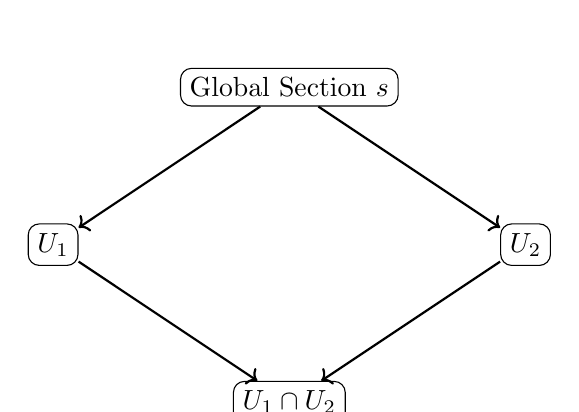
\begin{tikzpicture}[
		every node/.style={
			draw,
			rounded corners,
			align=center
		}
		]
		
		\node (u1) at (-3,0) {\(U_1\)};
		\node (u2) at (3,0) {\(U_2\)};
		\node (overlap) at (0,-2) {\(U_1\cap U_2\)};
		\node (global) at (0,2) {Global Section \(s\)};
		
		\draw[->,thick] (global)--(u1);
		\draw[->,thick] (global)--(u2);
		
		\draw[->,thick] (u1)--(overlap);
		\draw[->,thick] (u2)--(overlap);
		
	\end{tikzpicture}
\end{center}

The local sections must agree on overlaps before a global section can exist.

\subsection{Example: Continuous Functions Form a Sheaf}

Let

\[
U=U_1\cup U_2.
\]

Suppose

\[
f_1\in C(U_1),
\qquad
f_2\in C(U_2),
\]

and

\[
f_1=f_2
\]

on

\[
U_1\cap U_2.
\]

Then define

\[
f(x)=
\begin{cases}
	f_1(x), & x\in U_1,\\
	f_2(x), & x\in U_2.
\end{cases}
\]

The agreement on overlaps guarantees that \(f\) is continuous.

Thus

\[
C(-)
\]

is a sheaf.

\subsection{Counterexample: Bounded Continuous Functions}

Define

\[
\mathcal F(U)
=
\{f:U\to\mathbb R \mid f
\text{ continuous and bounded}\}.
\]

This is a presheaf.

Cover

\[
\mathbb R
=
\bigcup_{n=1}^{\infty}
(-n,n).
\]

For each \(n\),

\[
f_n(x)=x
\]

is bounded on \((-n,n)\).

These local sections agree on overlaps.

The glued function is

\[
f(x)=x.
\]

But \(f\) is not bounded on \(\mathbb R\).

Hence the glued section does not belong to

\[
\mathcal F(\mathbb R).
\]

Therefore

\[
\boxed{\mathcal F \text{ is not a sheaf.}}
\]

\subsection{Counterexample: Constant Functions}

Define

\[
\mathcal F(U)
=
\{\text{constant functions on }U\}.
\]

Take

\[
U=(-1,0)\cup(0,1).
\]

Define

\[
f_1=0
\]

on \((-1,0)\),

and

\[
f_2=1
\]

on \((0,1)\).

There is no overlap.

Compatibility is automatic.

The glued function becomes

\[
f=
\begin{cases}
	0,&x<0,\\
	1,&x>0.
\end{cases}
\]

which is not constant.

Hence constant functions form only a presheaf.

\subsection{Quotient Presheaves}

Suppose

\[
\mathcal G\subseteq \mathcal F
\]

is a sub-presheaf.

The quotient presheaf is

\[
(\mathcal F/\mathcal G)(U)
=
\mathcal F(U)/\mathcal G(U).
\]

\begin{example}
	Continuous functions modulo constants:
	
	\[
	C(U)/\mathbb R.
	\]
\end{example}

A quotient presheaf may fail to satisfy the sheaf axioms.

This motivates sheafification.

\subsection{Sheafification}

\begin{definition}
	For every presheaf \(\mathcal F\) there exists a sheaf
	
	\[
	\mathcal F^+
	\]
	
	and a morphism
	
	\[
	\mathcal F\to\mathcal F^+
	\]
	
	which is universal among all morphisms from \(\mathcal F\) to sheaves.
\end{definition}

Intuitively, sheafification:

\begin{itemize}
	\item keeps the local sections,
	\item identifies sections that agree locally,
	\item adds all missing glued sections.
\end{itemize}

\subsection{Germs}

Fix a point

\[
x\in X.
\]

Suppose

\[
s\in \mathcal F(U),
\qquad
t\in \mathcal F(V),
\]

where

\[
x\in U\cap V.
\]

\begin{definition}
	The sections \(s\) and \(t\) are equivalent at \(x\),
	
	\[
	s\sim_x t,
	\]
	
	if there exists a neighborhood
	
	\[
	W\subseteq U\cap V
	\]
	
	containing \(x\) such that
	
	\[
	s|_W=t|_W.
	\]
\end{definition}

The equivalence class

\[
[s]_x
\]

is called the \emph{germ} of \(s\) at \(x\).

\subsection{Intuition Behind Germs}

A germ remembers only what happens arbitrarily close to \(x\).

Everything away from \(x\) is ignored.

\[
\boxed{
	\text{Germ = local behavior near a point.}
}
\]

\subsection{Stalks}

\begin{definition}
	The stalk of a sheaf \(\mathcal F\) at \(x\) is
	
	\[
	\mathcal F_x
	=
	\varinjlim_{x\in U}
	\mathcal F(U).
	\]
\end{definition}

Equivalently,

\[
\boxed{
	\mathcal F_x
	=
	\{\text{all germs at }x\}.
}
\]

\subsection{Stalk as a Colimit}

The neighborhoods of \(x\)

\[
U_1 \supseteq U_2 \supseteq U_3 \supseteq \cdots
\]

form a directed system.

\begin{center}
	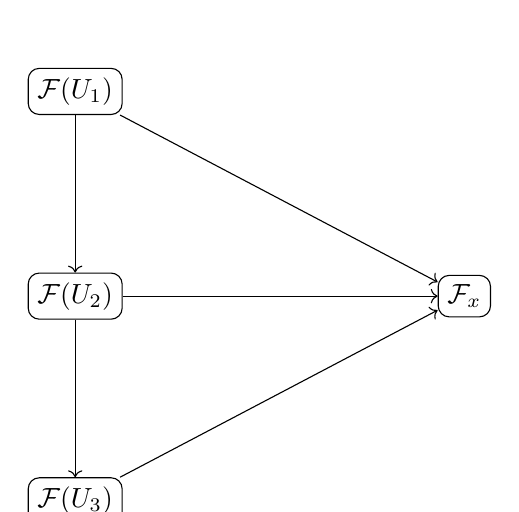
\begin{tikzpicture}[
		node distance=2cm,
		every node/.style={
			draw,
			rounded corners
		}
		]
		
		\node (u1) {\(\mathcal F(U_1)\)};
		\node (u2) [below=of u1] {\(\mathcal F(U_2)\)};
		\node (u3) [below=of u2] {\(\mathcal F(U_3)\)};
		\node (stalk) [right=4cm of u2] {\(\mathcal F_x\)};
		
		\draw[->] (u1)--(u2);
		\draw[->] (u2)--(u3);
		
		\draw[->] (u1)--(stalk);
		\draw[->] (u2)--(stalk);
		\draw[->] (u3)--(stalk);
		
	\end{tikzpicture}
\end{center}

The colimit identifies sections that become equal on some smaller neighborhood.

\subsection{Example of a Stalk}

Let

\[
\mathcal F(U)=C(U).
\]

At \(x=0\),

\[
f(x)=x
\]

and

\[
h(x)=
\begin{cases}
	x,& |x|<1,\\
	100,& |x|\ge 1
\end{cases}
\]

define the same germ.

Indeed, on a sufficiently small neighborhood of \(0\),

\[
f=h.
\]

Hence

\[
[f]_0=[h]_0.
\]

\subsection{Conceptual Hierarchy}

\begin{center}
	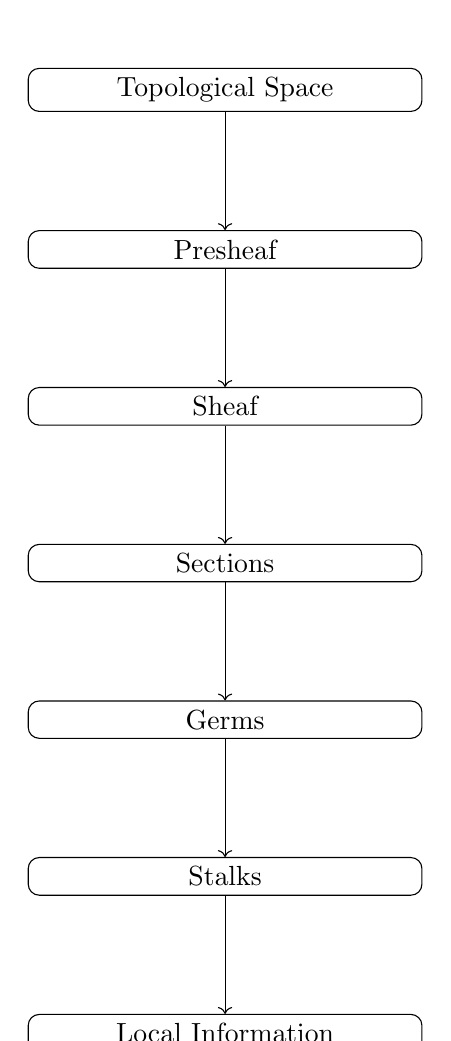
\begin{tikzpicture}[
		node distance=1.5cm,
		every node/.style={
			draw,
			rounded corners,
			minimum width=5cm,
			align=center
		}
		]
		
		\node (top) {Topological Space};
		
		\node (pre) [below=of top] {Presheaf};
		
		\node (sheaf) [below=of pre] {Sheaf};
		
		\node (sections) [below=of sheaf] {Sections};
		
		\node (germs) [below=of sections] {Germs};
		
		\node (stalks) [below=of germs] {Stalks};
		
		\node (local) [below=of stalks] {Local Information};
		
		\draw[->] (top)--(pre);
		\draw[->] (pre)--(sheaf);
		\draw[->] (sheaf)--(sections);
		\draw[->] (sections)--(germs);
		\draw[->] (germs)--(stalks);
		\draw[->] (stalks)--(local);
		
	\end{tikzpicture}
\end{center}

\subsection{Fundamental Principle}

\[
\boxed{
	\text{Presheaf = local objects with restrictions.}
}
\]

\[
\boxed{
	\text{Sheaf = local objects that glue uniquely.}
}
\]

\[
\boxed{
	\text{Germ = local behavior at one point.}
}
\]

\[
\boxed{
	\text{Stalk = the set of all germs at that point.}
}
\]

\[
\boxed{
	\mathcal F_x
	=
	\varinjlim_{x\in U}
	\mathcal F(U).
}
\]

The language of sheaves and stalks is one of the central foundations of modern algebraic geometry, complex geometry, differential geometry, cohomology theory, and the theory of schemes.	
	
\subsection{Additional Examples of Quotient Sheaves}

Quotient sheaves arise whenever a sheaf contains a subsheaf and we identify sections differing by elements of that subsheaf.

\bigskip

Let

\[
\mathcal G\subseteq \mathcal F
\]

be a subsheaf.

The quotient sheaf is denoted

\[
\mathcal F/\mathcal G.
\]

For each open set \(U\),

\[
(\mathcal F/\mathcal G)(U)
=
\mathcal F(U)/\mathcal G(U)
\]

followed (if necessary) by sheafification.

\subsubsection*{Example 1: Continuous Functions Modulo Constants}

Let

\[
\underline{\mathbb R}
\]

denote the constant sheaf.

Consider

\[
\mathcal C/\underline{\mathbb R}.
\]

For an open set \(U\),

\[
(\mathcal C/\underline{\mathbb R})(U)
=
C(U)/\mathbb R.
\]

Two functions are identified whenever they differ by a constant:

\[
f\sim g
\quad\Longleftrightarrow\quad
f-g=c.
\]

For example,

\[
x^2
\]

and

\[
x^2+5
\]

represent the same section.

This quotient remembers only changes in the function and ignores vertical translations.

\bigskip

\subsubsection*{Example 2: Holomorphic Functions Modulo Constants}

On a complex manifold let

\[
\mathcal O
\]

be the sheaf of holomorphic functions.

Then

\[
\mathcal O/\underline{\mathbb C}
\]

identifies holomorphic functions differing by constants.

Thus

\[
z^2
\]

and

\[
z^2+7
\]

represent the same class.

This quotient appears naturally when studying differentials because

\[
d(f+c)=df.
\]

\bigskip

\subsubsection*{Example 3: Functions Modulo Vanishing Functions}

Fix a point

\[
p\in X.
\]

Let

\[
\mathfrak m_p(U)
=
\{f\in\mathcal O(U)\mid f(p)=0\}.
\]

Then

\[
\mathcal O_p/\mathfrak m_p
\]

is called the residue field at \(p\).

For complex varieties:

\[
\mathcal O_p/\mathfrak m_p
\cong
\mathbb C.
\]

This quotient remembers only the value of a function at the point \(p\).

Indeed,

\[
f
\equiv
g
\pmod{\mathfrak m_p}
\]

iff

\[
f(p)=g(p).
\]

\bigskip

\subsubsection*{Example 4: First-Order Infinitesimal Quotient}

Let

\[
\mathfrak m_p
\]

be the maximal ideal of functions vanishing at \(p\).

Consider

\[
\mathfrak m_p/\mathfrak m_p^2.
\]

This quotient forgets all quadratic and higher-order terms.

For

\[
f(x)=3x+5x^2+x^3,
\]

the class of \(f\) in

\[
\mathfrak m_p/\mathfrak m_p^2
\]

is represented simply by

\[
3x.
\]

This space is dual to the tangent space:

\[
T_p^*X
\cong
\mathfrak m_p/\mathfrak m_p^2.
\]

It is one of the most important quotients in algebraic geometry.

\bigskip

\subsubsection*{Example 5: Differential Forms Modulo Exact Forms}

Let

\[
\Omega^1
\]

be the sheaf of differential \(1\)-forms.

Let

\[
d\mathcal O
\]

denote the image of

\[
d:\mathcal O\to\Omega^1.
\]

Then

\[
\Omega^1/d\mathcal O
\]

identifies forms differing by an exact form.

For example,

\[
(x\,dx)
\]

and

\[
(x\,dx+d(x^2))
\]

represent the same class.

Such quotients lead naturally to de Rham cohomology.

\bigskip

\subsubsection*{Example 6: Rational Functions Modulo Regular Functions}

Let

\[
\mathcal K
\]

be the sheaf of rational functions on a variety.

Since

\[
\mathcal O\subseteq \mathcal K,
\]

we may form

\[
\mathcal K/\mathcal O.
\]

A section records only the poles of a rational function.

For instance,

\[
\frac1x
\]

defines a nontrivial class because it is not regular at \(x=0\).

This quotient plays a central role in divisor theory.

\bigskip

\subsubsection*{Example 7: The Exponential Sequence Quotient}

Consider the exponential map

\[
\exp(2\pi i\cdot):
\mathcal O
\to
\mathcal O^\times.
\]

Its kernel is

\[
\underline{\mathbb Z}.
\]

Thus there is an exact sequence

\[
0
\to
\underline{\mathbb Z}
\to
\mathcal O
\to
\mathcal O^\times
\to
0.
\]

Here

\[
\mathcal O^\times
\cong
\mathcal O/\underline{\mathbb Z}
\]

(after interpreting the quotient appropriately through the exact sequence).

This leads directly to line bundles and Chern classes.

\bigskip

\subsection{Geometric Interpretation of Important Quotients}

\begin{center}
	\renewcommand{\arraystretch}{1.4}
	\begin{tabular}{|p{4cm}|p{5cm}|p{5cm}|}
		\hline
		Quotient & What Is Forgotten & What Remains \\
		\hline
		
		\(C/\mathbb R\)
		&
		Constant shifts
		&
		Relative shape
		\\
		\hline
		
		\(\mathcal O/\mathbb C\)
		&
		Constant terms
		&
		Holomorphic variation
		\\
		\hline
		
		\(\mathcal O_p/\mathfrak m_p\)
		&
		Everything except value
		&
		Function value at \(p\)
		\\
		\hline
		
		\(\mathfrak m_p/\mathfrak m_p^2\)
		&
		Quadratic and higher terms
		&
		Linear information
		\\
		\hline
		
		\(\Omega^1/d\mathcal O\)
		&
		Exact forms
		&
		Cohomological information
		\\
		\hline
		
		\(\mathcal K/\mathcal O\)
		&
		Regular part
		&
		Pole structure
		\\
		\hline
		
	\end{tabular}
\end{center}	
	
\end{document}

